\documentclass[11pt]{article}
\usepackage{fullpage}
\usepackage{fancyhdr}

\usepackage{amsmath}
\usepackage{amssymb}
\usepackage{url}

\usepackage{listings}
\usepackage{color}
\lstset{language=Python,
        basicstyle=\footnotesize\ttfamily,
        showspaces=false,
        showstringspaces=false,
        tabsize=2,
        breaklines=false,
        breakatwhitespace=true,
        identifierstyle=\ttfamily,
        keywordstyle=\color[rgb]{0,0,1},
        commentstyle=\color[rgb]{0.133,0.545,0.133},
        stringstyle=\color[rgb]{0.627,0.126,0.941},
    }

\usepackage[pdftex]{graphicx}

% header
\fancyhead{}
\fancyfoot{}
\fancyfoot[C]{\thepage}
\fancyhead[R]{Daniel Foreman-Mackey}
\fancyhead[L]{Statistical Natural Language Processing --- Homework 2}
\pagestyle{fancy}
\setlength{\headsep}{10pt}
\setlength{\headheight}{20pt}

% shortcuts
\newcommand{\Eq}[1]{Equation (\ref{eq:#1})}
\newcommand{\eq}[1]{Equation (\ref{eq:#1})}
\newcommand{\eqlabel}[1]{\label{eq:#1}}
\newcommand{\Fig}[1]{Figure \ref{fig:#1}}
\newcommand{\fig}[1]{Figure \ref{fig:#1}}
\newcommand{\figlabel}[1]{\label{fig:#1}}

\newcommand{\pr}[1]{\ensuremath{p\left (#1 \right )}}
\newcommand{\lk}[1]{\ensuremath{\mathcal{L} \left ( #1 \right )}}
\newcommand{\bvec}[1]{\ensuremath{\boldsymbol{#1}}}
\newcommand{\dd}{\ensuremath{\, \mathrm{d}}}
\newcommand{\normal}[2]{\ensuremath{\mathcal{N} \left ( #1; #2 \right ) }}

\newcommand{\data}{\mathcal{D}}

\newcommand{\code}[1]{{\sffamily #1}}


\begin{document}

The goal of this project is to classify a noun into one of five categories
(\code{place}, \code{movie}, \code{drug}, \code{person}, or \code{company})
using only the word itself.
I'll focus on building a discriminative model based on logistic regression.

\section{A note about implementation}

Instead of using the provided Java code, I decided to implement my assignment
in Python and C.
The data manipulation and feature extraction is all performed in Python using
the standard library.
Once the feature vectors have been built, they are passed to the C code that
does the computationally heavy lifting.
The standard Python implementation of \code{BFGS} was not efficient enough for
the purposes of this assignment so I used the \code{libLBFGS}%
\footnote{\url{http://www.chokkan.org/software/liblbfgs/}} C implementation
of the \code{L-BFGS} algorithm.
All of the code used in this assignment is available on GitHub at:
\url{https://github.com/dfm/stat-nlp-nyu}.

\section{Discriminative proper noun classification with logistic regression}

\begin{figure}[htbp]
\begin{center}
    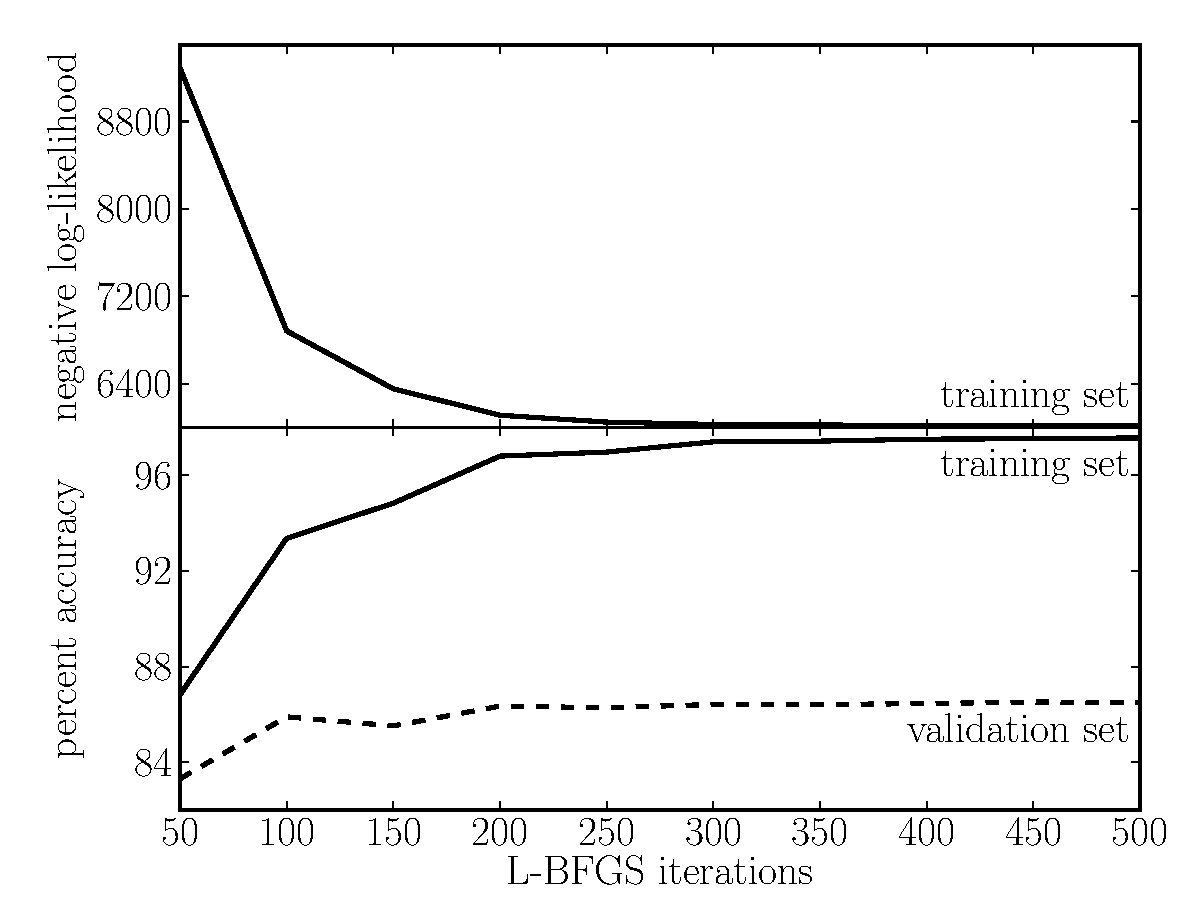
\includegraphics[width=\textwidth]{full_500_convergence.pdf}
\end{center}
\caption{%
\figlabel{full500}}
\end{figure}

\end{document}
